\documentclass[aspectratio=169]{beamer}

\usetheme{default}
\usecolortheme{default}
\usefonttheme{professionalfonts}

\usepackage[T1]{fontenc}
\usepackage{lmodern}
\usepackage{tikz}
\usepackage{booktabs}
\usepackage{array}
\usepackage{tabularx}
\usepackage{graphicx}
\usetikzlibrary{positioning,arrows.meta,calc,fit,shapes.geometric}

\definecolor{MemphisBlue}{RGB}{26,62,122}
\definecolor{LightBand}{RGB}{244,247,252}
\definecolor{MidBand}{RGB}{229,236,247}
\definecolor{SoftGray}{RGB}{90,96,108}
\definecolor{AccentGreen}{RGB}{61,130,89}
\definecolor{AccentOrange}{RGB}{194,111,46}
\definecolor{AccentRed}{RGB}{168,65,65}

\setbeamertemplate{navigation symbols}{}
\setbeamertemplate{itemize item}{\color{MemphisBlue}$\blacktriangleright$}
\setbeamertemplate{itemize subitem}{\color{MemphisBlue}$\circ$}
\setbeamercolor{title}{fg=MemphisBlue}
\setbeamercolor{frametitle}{fg=MemphisBlue,bg=white}
\setbeamercolor{author in head/foot}{fg=MemphisBlue,bg=white}
\setbeamercolor{date in head/foot}{fg=MemphisBlue,bg=white}
\setbeamercolor{block body}{bg=LightBand,fg=black}
\setbeamerfont{frametitle}{size=\Large,series=\bfseries}
\setbeamerfont{title}{size=\LARGE,series=\bfseries}
\setbeamerfont{subtitle}{size=\large}
\setbeamerfont{normal text}{size=\normalsize}

\setbeamertemplate{footline}{%
  \leavevmode%
  \hbox{%
    \begin{beamercolorbox}[wd=.76\paperwidth,ht=2.6ex,dp=1.2ex,leftskip=1.2em]{author in head/foot}%
      \scriptsize NDNSF-UAV-APP: Design and Mechanisms
    \end{beamercolorbox}%
    \begin{beamercolorbox}[wd=.24\paperwidth,ht=2.6ex,dp=1.2ex,rightskip=1.2em plus1fil]{date in head/foot}%
      \scriptsize \insertframenumber/\inserttotalframenumber
    \end{beamercolorbox}%
  }%
}

\newcommand{\bluebox}[1]{%
  \begin{beamercolorbox}[rounded=true,shadow=false,sep=0.65em,wd=0.94\linewidth]{block body}
  #1
  \end{beamercolorbox}
}

\newcommand{\evidence}[1]{%
  \vfill\par\noindent
  \begin{minipage}{\linewidth}
  \raggedright{\color{SoftGray}\tiny Evidence: #1}\par
  \end{minipage}
}

\newcolumntype{Y}{>{\raggedright\arraybackslash}X}

\tikzset{
  flow/.style={-{Stealth[length=2.2mm]},thick,draw=MemphisBlue},
  backflow/.style={{Stealth[length=2.2mm]}-,thick,draw=MemphisBlue},
  dashflow/.style={-{Stealth[length=2.2mm]},thick,dashed,draw=AccentOrange},
  thinflow/.style={-{Stealth[length=1.8mm]},semithick,draw=MemphisBlue},
  box/.style={draw=MemphisBlue,fill=LightBand,rounded corners=2pt,
    minimum height=0.72cm,align=center,font=\scriptsize},
  strongbox/.style={draw=MemphisBlue,fill=MidBand,rounded corners=2pt,
    minimum height=0.78cm,align=center,font=\scriptsize\bfseries},
  greenbox/.style={draw=AccentGreen,fill=AccentGreen!10,rounded corners=2pt,
    minimum height=0.72cm,align=center,font=\scriptsize},
  orangebox/.style={draw=AccentOrange,fill=AccentOrange!10,rounded corners=2pt,
    minimum height=0.72cm,align=center,font=\scriptsize},
  redbox/.style={draw=AccentRed,fill=AccentRed!8,rounded corners=2pt,
    minimum height=0.72cm,align=center,font=\scriptsize}
}

\title{NDNSF-UAV-APP}
\subtitle{Named Services for Secure Control, Adaptive Video, and Multi-Drone Operations}
\author{Tianxing Ma}
\institute{Department of Computer Science\\University of Memphis}
\date{July 2026}

\begin{document}

\begin{frame}[plain]
  \titlepage
\end{frame}

\begin{frame}{Why an NDN-Native UAV Application?}
\footnotesize
\begin{columns}[T]
\begin{column}{0.48\textwidth}
\textbf{One mission combines different communication needs}
\begin{itemize}
  \item Safety-sensitive commands need authorization and prompt failure.
  \item Telemetry and readiness must stay tied to the selected vehicle.
  \item Live video and retained playback share canonical Data; exported files and logs are durable objects.
  \item Multiple mobile drones may be busy, disconnected, or replaceable.
\end{itemize}
\end{column}
\begin{column}{0.48\textwidth}
\begin{center}
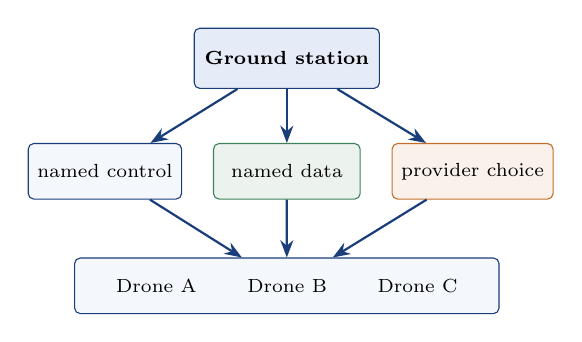
\begin{tikzpicture}[node distance=0.45cm,scale=0.98,transform shape]
  \node[strongbox,minimum width=2.4cm] (gs) {Ground station};
  \node[box,below left=0.7cm and 0.15cm of gs,minimum width=1.9cm] (control) {named control};
  \node[greenbox,below=0.7cm of gs,minimum width=1.9cm] (data) {named data};
  \node[orangebox,below right=0.7cm and 0.15cm of gs,minimum width=1.9cm] (select) {provider choice};
  \node[box,below=0.75cm of data,minimum width=5.5cm] (drones) {Drone A \qquad Drone B \qquad Drone C};
  \draw[flow] (gs) -- (control);
  \draw[flow] (gs) -- (data);
  \draw[flow] (gs) -- (select);
  \draw[flow] (control) -- (drones);
  \draw[flow] (data) -- (drones);
  \draw[flow] (select) -- (drones);
\end{tikzpicture}
\end{center}
\end{column}
\end{columns}

\vspace{0.4em}
\bluebox{The application binds UAV operations to \textbf{service and data names}, not to one fixed endpoint connection.}
\evidence{NDNSF-UAV-APP/README.md: Why This Application Exists}
\end{frame}

\begin{frame}{Responsibility Boundary}
\footnotesize
\begin{center}
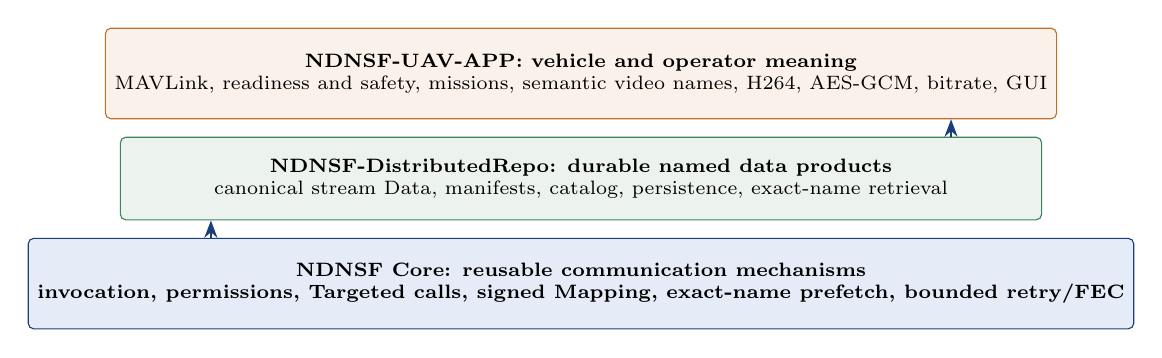
\begin{tikzpicture}[node distance=0.3cm]
  \node[orangebox,minimum width=11.7cm,minimum height=1.15cm] (app) {
    \textbf{NDNSF-UAV-APP: vehicle and operator meaning}\\
    MAVLink, readiness and safety, missions, semantic video names, H264, AES-GCM, bitrate, GUI
  };
  \node[greenbox,below=0.22cm of app,minimum width=11.7cm,minimum height=1.05cm] (repo) {
    \textbf{NDNSF-DistributedRepo: durable named data products}\\
    canonical stream Data, manifests, catalog, persistence, exact-name retrieval
  };
  \node[strongbox,below=0.22cm of repo,minimum width=11.7cm,minimum height=1.15cm] (core) {
    \textbf{NDNSF Core: reusable communication mechanisms}\\
    invocation, permissions, Targeted calls, signed Mapping, exact-name prefetch, bounded retry/FEC
  };
  \draw[flow] ([xshift=-4.7cm]core.north) -- ([xshift=-4.7cm]repo.south);
  \draw[flow] ([xshift=4.7cm]repo.north) -- ([xshift=4.7cm]app.south);
\end{tikzpicture}
\end{center}

\vspace{0.25em}
\bluebox{Core transports opaque bytes under application names; UAV owns video meaning and encryption, while Core owns the reusable live network loop.}
\evidence{docs/ndnsf-core-app-boundary.md; Spec 118/119 ownership contracts}
\end{frame}

\begin{frame}{Three Runtime Roles}
\footnotesize
\begin{center}
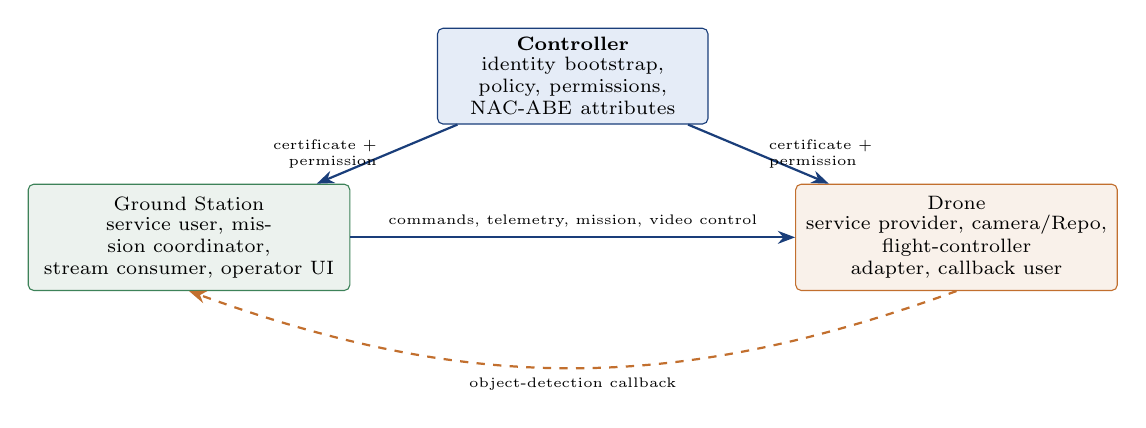
\begin{tikzpicture}[node distance=0.55cm]
  \node[strongbox,text width=3.2cm,minimum height=1.15cm] (controller) {
    Controller\\[-0.1em]
    \normalfont identity bootstrap, policy, permissions, NAC-ABE attributes
  };
  \node[greenbox,below left=0.75cm and 1.1cm of controller,text width=3.85cm,minimum height=1.35cm] (gs) {
    Ground Station\\[-0.1em]
    \normalfont service user, mission coordinator,\\stream consumer, operator UI
  };
  \node[orangebox,below right=0.75cm and 1.1cm of controller,text width=3.85cm,minimum height=1.35cm] (drone) {
    Drone\\[-0.1em]
    \normalfont service provider, camera/Repo,\\flight-controller adapter, callback user
  };
  \draw[flow] (controller) -- node[left,font=\tiny,align=right] {certificate +\\permission} (gs);
  \draw[flow] (controller) -- node[right,font=\tiny,align=left] {certificate +\\permission} (drone);
  \draw[flow] (gs) -- node[above,font=\tiny] {commands, telemetry, mission, video control} (drone);
  \draw[dashflow] (drone.south) to[bend left=20] node[below,font=\tiny] {object-detection callback} (gs.south);
\end{tikzpicture}
\end{center}

\vspace{0.35em}
\begin{columns}[T]
\begin{column}{0.48\textwidth}
\textbf{Typical PC}: Controller + Ground Station + NFD
\end{column}
\begin{column}{0.48\textwidth}
\textbf{Each vehicle}: DroneAPP + NFD + camera + MAVLink link
\end{column}
\end{columns}
\evidence{UavDroneApp.cpp; UavGroundStationApp.cpp; README deployment section}
\end{frame}

\begin{frame}{Service Containers, Not One Monolithic RPC}
\footnotesize
\begin{columns}[T]
\begin{column}{0.49\textwidth}
\begin{center}
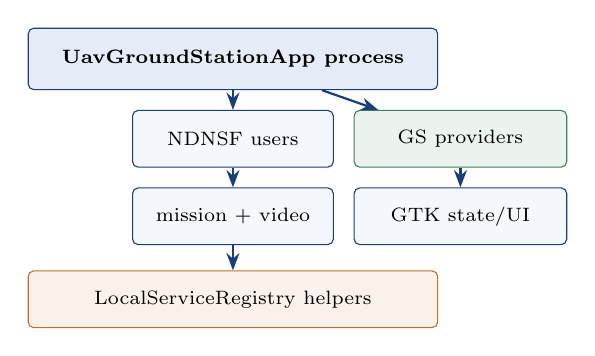
\begin{tikzpicture}[node distance=0.25cm]
  \node[strongbox,minimum width=5.2cm] (gsprocess) {UavGroundStationApp process};
  \node[box,below=of gsprocess,minimum width=2.55cm] (users) {NDNSF users};
  \node[greenbox,right=0.25cm of users,minimum width=2.7cm] (gsprovider) {GS providers};
  \node[box,below=of users,minimum width=2.55cm] (workflow) {mission + video};
  \node[box,right=0.25cm of workflow,minimum width=2.7cm] (gui) {GTK state/UI};
  \node[orangebox,below=0.32cm of workflow,minimum width=5.2cm] (gslocal) {LocalServiceRegistry helpers};
  \draw[flow] (gsprocess) -- (users);
  \draw[flow] (gsprocess) -- (gsprovider);
  \draw[flow] (users) -- (workflow);
  \draw[flow] (gsprovider) -- (gui);
  \draw[flow] (workflow) -- (gslocal);
\end{tikzpicture}
\end{center}
\end{column}
\begin{column}{0.49\textwidth}
\begin{center}
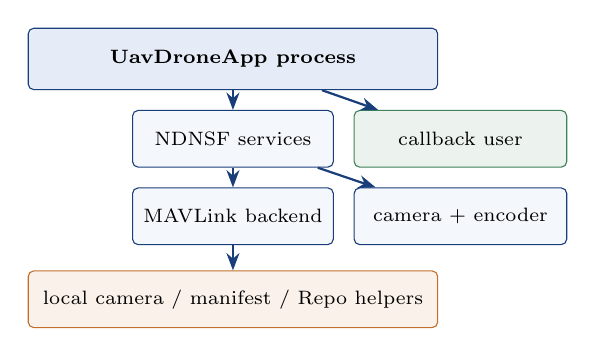
\begin{tikzpicture}[node distance=0.25cm]
  \node[strongbox,minimum width=5.2cm] (droneprocess) {UavDroneApp process};
  \node[box,below=of droneprocess,minimum width=2.55cm] (providers) {NDNSF services};
  \node[greenbox,right=0.25cm of providers,minimum width=2.7cm] (callback) {callback user};
  \node[box,below=of providers,minimum width=2.55cm] (mav) {MAVLink backend};
  \node[box,right=0.25cm of mav,minimum width=2.7cm] (camera) {camera + encoder};
  \node[orangebox,below=0.32cm of mav,minimum width=5.2cm] (local) {local camera / manifest / Repo helpers};
  \draw[flow] (droneprocess) -- (providers);
  \draw[flow] (droneprocess) -- (callback);
  \draw[flow] (providers) -- (mav);
  \draw[flow] (providers) -- (camera);
  \draw[flow] (mav) -- (local);
\end{tikzpicture}
\end{center}
\end{column}
\end{columns}

\vspace{0.35em}
\bluebox{One process shares identity, configuration, hardware, and lifecycle; every remote service remains separately named and permission-controlled.}
\evidence{DroneServiceContainer.inc.hpp; GroundStationServiceContainer.inc.hpp}
\end{frame}

\begin{frame}{Named Services and Invocation Modes}
\scriptsize
\renewcommand{\arraystretch}{1.12}
\begin{tabularx}{\textwidth}{>{\ttfamily}p{4.6cm} p{2.7cm} Y}
\toprule
\textbf{Name} & \textbf{Mode} & \textbf{Purpose} \\
\midrule
/UAV/MAVLink/Execute & Targeted only & known-drone low-latency command path \\
/UAV/Telemetry/GetStatus & normal +\newline Targeted & discovery or selected-drone state refresh \\
/UAV/Mission/Assign & normal & multi-provider mission-slot selection \\
/<drone>/UAV/Camera/Video & normal & provider-specific Start/Stop control \\
/<drone>/UAV/MAVLink/\newline Parameters & normal & vehicle capability and parameter snapshot \\
/<drone>/UAV/Preflight/\newline Checklist & normal & typed operator readiness details \\
/<drone>/UAV/Camera/\newline Recording/Manifest & normal & discover retained canonical stream Data \\
/UAV/GS/ObjectDetection & normal & drone-to-ground-station compute callback \\
\bottomrule
\end{tabularx}

\vspace{0.35em}
\bluebox{Shared service names allow provider selection; provider-specific names address one physical vehicle or its data product.}
\evidence{shared/UavNames.hpp; DroneServiceContainer::installServiceInstances}
\end{frame}

\begin{frame}{Secure Startup and Invocation}
\footnotesize
\begin{center}
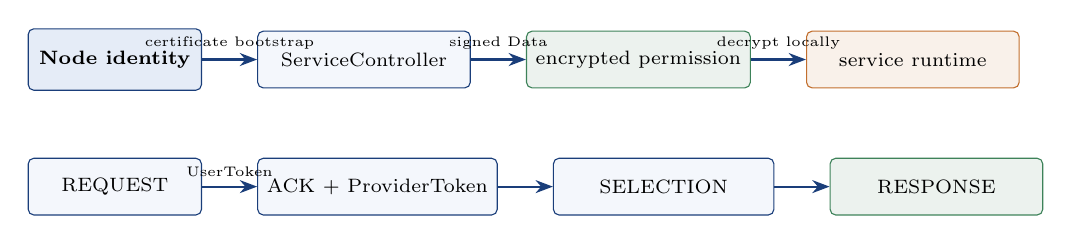
\begin{tikzpicture}[node distance=0.55cm]
  \node[strongbox,minimum width=2.2cm] (identity) {Node identity};
  \node[box,right=0.7cm of identity,minimum width=2.7cm] (controller) {ServiceController};
  \node[greenbox,right=0.7cm of controller,minimum width=2.8cm] (permission) {encrypted permission};
  \node[orangebox,right=0.7cm of permission,minimum width=2.7cm] (runtime) {service runtime};
  \draw[flow] (identity) -- node[above,font=\tiny] {certificate bootstrap} (controller);
  \draw[flow] (controller) -- node[above,font=\tiny] {signed Data} (permission);
  \draw[flow] (permission) -- node[above,font=\tiny] {decrypt locally} (runtime);

  \node[box,below=0.85cm of identity,minimum width=2.2cm] (req) {REQUEST};
  \node[box,right=0.7cm of req,minimum width=2.7cm] (ack) {ACK + ProviderToken};
  \node[box,right=0.7cm of ack,minimum width=2.8cm] (sel) {SELECTION};
  \node[greenbox,right=0.7cm of sel,minimum width=2.7cm] (resp) {RESPONSE};
  \draw[flow] (req) -- node[above,font=\tiny] {UserToken} (ack);
  \draw[flow] (ack) -- (sel);
  \draw[flow] (sel) -- (resp);
\end{tikzpicture}
\end{center}

\vspace{0.55em}
\begin{itemize}
  \item REQUEST/SELECTION use service attributes; ACK/RESPONSE use permission attributes.
  \item One-time user/provider tokens bind the handshake and reject replay.
  \item Controller permission Data is signed and encrypted to the target identity certificate.
\end{itemize}
\evidence{ServiceController; ServiceUser/ServiceProvider security path; UAV deployment README}
\end{frame}

\begin{frame}{Targeted MAVLink Command Path}
\footnotesize
\begin{center}
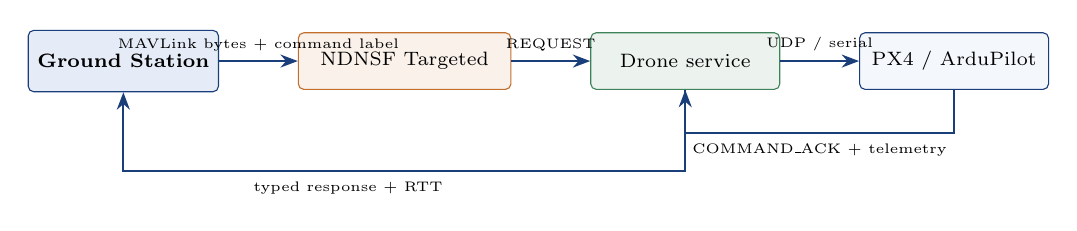
\begin{tikzpicture}[node distance=0.65cm]
  \node[strongbox,minimum width=2.4cm] (gs) {Ground Station};
  \node[orangebox,right=1.0cm of gs,minimum width=2.7cm] (ndnsf) {NDNSF Targeted};
  \node[greenbox,right=1.0cm of ndnsf,minimum width=2.4cm] (drone) {Drone service};
  \node[box,right=1.0cm of drone,minimum width=2.4cm] (fc) {PX4 / ArduPilot};
  \draw[flow] (gs) -- node[above,font=\tiny] {MAVLink bytes + command label} (ndnsf);
  \draw[flow] (ndnsf) -- node[above,font=\tiny] {REQUEST} (drone);
  \draw[flow] (drone) -- node[above,font=\tiny] {UDP / serial} (fc);
  \draw[backflow] (drone.south) -- ++(0,-0.55cm) -| node[below,pos=0.25,font=\tiny] {COMMAND\_ACK + telemetry} (fc.south);
  \draw[backflow] (gs.south) -- ++(0,-1.0cm) -| node[below,pos=0.2,font=\tiny] {typed response + RTT} (drone.south);
\end{tikzpicture}
\end{center}

\vspace{0.55em}
\begin{columns}[T]
\begin{column}{0.48\textwidth}
\textbf{First use}
\begin{itemize}
  \item authenticated ACK/selection bootstrap
  \item obtain a batch of one-time token pairs
\end{itemize}
\end{column}
\begin{column}{0.48\textwidth}
\textbf{Later commands}
\begin{itemize}
  \item request/response-only Targeted calls
  \item permissions, token checks, and replay protection remain
\end{itemize}
\end{column}
\end{columns}
\evidence{sendMavlinkCommandToDrone; ServiceProvider TargetedOnly registration}
\end{frame}

\begin{frame}{Typed State Drives the Operator Workflow}
\footnotesize
\begin{columns}[T]
\begin{column}{0.56\textwidth}
\begin{center}
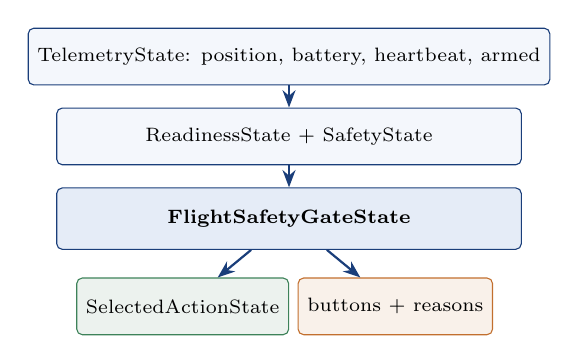
\begin{tikzpicture}[node distance=0.28cm]
  \node[box,minimum width=5.9cm] (telemetry) {TelemetryState: position, battery, heartbeat, armed};
  \node[box,below=of telemetry,minimum width=5.9cm] (readiness) {ReadinessState + SafetyState};
  \node[strongbox,below=of readiness,minimum width=5.9cm] (gate) {FlightSafetyGateState};
  \node[greenbox,below=0.35cm of gate,xshift=-1.35cm,minimum width=2.4cm] (actions) {SelectedActionState};
  \node[orangebox,below=0.35cm of gate,xshift=1.35cm,minimum width=2.4cm] (ui) {buttons + reasons};
  \draw[flow] (telemetry) -- (readiness);
  \draw[flow] (readiness) -- (gate);
  \draw[flow] (gate) -- (actions);
  \draw[flow] (gate) -- (ui);
\end{tikzpicture}
\end{center}
\end{column}
\begin{column}{0.41\textwidth}
\textbf{Command lifecycle}
\begin{center}
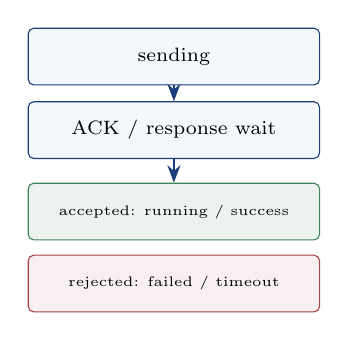
\begin{tikzpicture}[node distance=0.2cm]
  \node[box,minimum width=3.7cm] (send) {sending};
  \node[box,below=of send,minimum width=3.7cm] (wait) {ACK / response wait};
  \node[greenbox,below=0.3cm of wait,minimum width=3.7cm,font=\tiny] (ok) {accepted: running / success};
  \node[redbox,below=0.18cm of ok,minimum width=3.7cm,font=\tiny] (bad) {rejected: failed / timeout};
  \draw[flow] (send) -- (wait);
  \draw[flow] (wait) -- (ok);
\end{tikzpicture}
\end{center}
\end{column}
\end{columns}

\vspace{0.35em}
\bluebox{The GUI reads typed state. Stale or lost telemetry changes the same safety model used by the actual command-send path.}
\evidence{shared/UavProtocol.hpp; GroundStationRuntimeState.hpp; commandLifecycle}
\end{frame}

\begin{frame}{Safety Gates and Operator Authority}
\footnotesize
\begin{center}
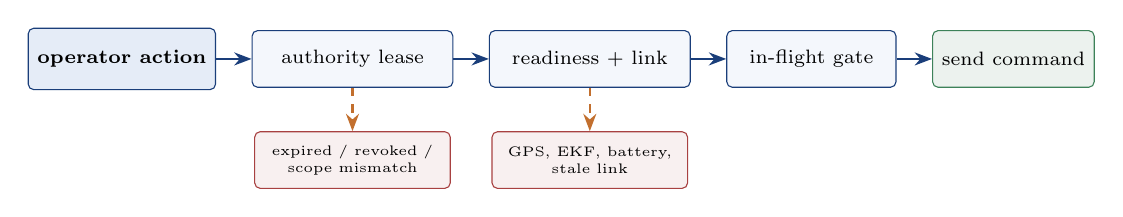
\begin{tikzpicture}[node distance=0.35cm]
  \node[strongbox,minimum width=2.3cm] (intent) {operator action};
  \node[box,right=0.45cm of intent,minimum width=2.55cm] (lease) {authority lease};
  \node[box,right=0.45cm of lease,minimum width=2.55cm] (ready) {readiness + link};
  \node[box,right=0.45cm of ready,minimum width=2.15cm] (busy) {in-flight gate};
  \node[greenbox,right=0.45cm of busy,minimum width=2.0cm] (send) {send command};
  \draw[flow] (intent) -- (lease);
  \draw[flow] (lease) -- (ready);
  \draw[flow] (ready) -- (busy);
  \draw[flow] (busy) -- (send);
  \node[redbox,below=0.55cm of lease,text width=2.25cm,font=\tiny] (deny1) {expired / revoked /\\scope mismatch};
  \node[redbox,below=0.55cm of ready,text width=2.25cm,font=\tiny] (deny2) {GPS, EKF, battery,\\stale link};
  \draw[dashflow] (lease) -- (deny1);
  \draw[dashflow] (ready) -- (deny2);
\end{tikzpicture}
\end{center}

\vspace{0.55em}
\begin{itemize}
  \item A lease binds operator, drone set, monitor/control scope, and time window.
  \item Monitor authority permits observation but does not permit flight control.
  \item Authority never overrides readiness or safety; both gates must pass.
  \item Rejection reasons and authority alerts remain visible and auditable.
\end{itemize}
\evidence{OperatorAuthorityLease; validateOperatorLease; validateFlightSafetyGate}
\end{frame}

\begin{frame}{Flight-Controller Adapter Boundary}
\footnotesize
\begin{columns}[T]
\begin{column}{0.49\textwidth}
\begin{center}
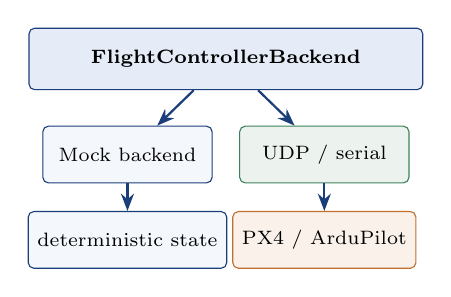
\begin{tikzpicture}[node distance=0.3cm]
  \node[strongbox,minimum width=5.0cm] (interface) {FlightControllerBackend};
  \node[box,below=0.45cm of interface,xshift=-1.25cm,minimum width=2.15cm] (mock) {Mock backend};
  \node[greenbox,below=0.45cm of interface,xshift=1.25cm,minimum width=2.15cm] (real) {UDP / serial};
  \node[box,below=0.35cm of mock,minimum width=2.15cm] (det) {deterministic state};
  \node[orangebox,below=0.35cm of real,minimum width=2.15cm] (px4) {PX4 / ArduPilot};
  \draw[flow] (interface) -- (mock);
  \draw[flow] (interface) -- (real);
  \draw[flow] (mock) -- (det);
  \draw[flow] (real) -- (px4);
\end{tikzpicture}
\end{center}
\end{column}
\begin{column}{0.47\textwidth}
\textbf{Backend contract}
\begin{itemize}
  \item forward MAVLink frames
  \item return command ACK fields
  \item expose latest telemetry
  \item read/edit parameters
  \item upload mission waypoints
\end{itemize}

\textbf{Real-link helpers}
\begin{itemize}
  \item GCS heartbeat
  \item manual-control replay
  \item neutral command after timeout
\end{itemize}
\end{column}
\end{columns}
\evidence{FlightControllerBackend; MockFlightControllerBackend; UdpFlightControllerBackend}
\end{frame}

\begin{frame}{Multi-Drone Mission Lifecycle}
\footnotesize
\begin{center}
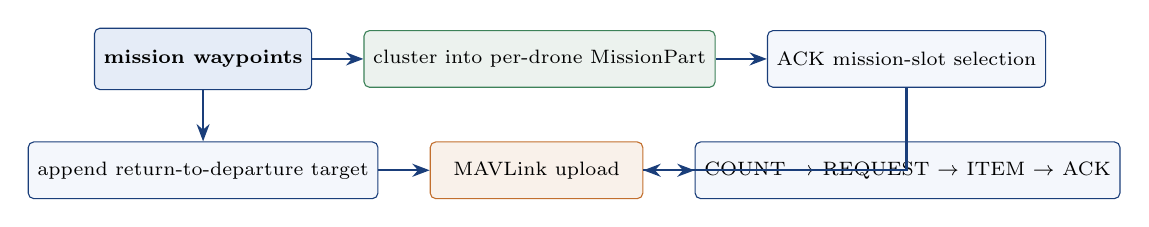
\begin{tikzpicture}[node distance=0.3cm]
  \node[strongbox,minimum width=2.5cm] (route) {mission waypoints};
  \node[greenbox,right=0.65cm of route,minimum width=3.7cm] (parts) {cluster into per-drone MissionPart};
  \node[box,right=0.65cm of parts,minimum width=3.2cm] (assign) {ACK mission-slot selection};
  \draw[flow] (route) -- (parts);
  \draw[flow] (parts) -- (assign);

  \node[box,below=0.65cm of route,minimum width=3.25cm] (return) {append return-to-departure target};
  \node[orangebox,right=0.65cm of return,minimum width=2.7cm] (upload) {MAVLink upload};
  \node[box,right=0.65cm of upload,minimum width=4.0cm] (handshake) {COUNT $\rightarrow$ REQUEST $\rightarrow$ ITEM $\rightarrow$ ACK};
  \draw[flow] (route) -- (return);
  \draw[flow] (assign) |- (upload);
  \draw[flow] (return) -- (upload);
  \draw[flow] (upload) -- (handshake);
\end{tikzpicture}
\end{center}

\vspace{0.55em}
\bluebox{Mission start is phased: arm accepted drones, take off accepted drones, then start only the mission parts that were uploaded successfully.}
\evidence{MissionPlan/MissionPart; uploadMissionPlan; executeMissionWaypoints}
\end{frame}

\begin{frame}{Mission Recovery and Persistence}
\footnotesize
\begin{columns}[T]
\begin{column}{0.49\textwidth}
\textbf{Application-level compensation}
\begin{center}
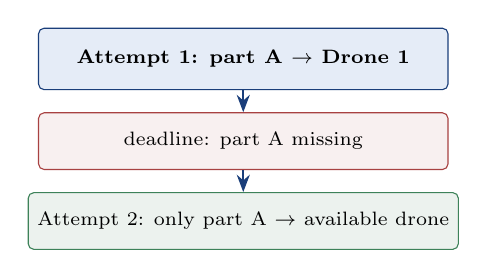
\begin{tikzpicture}[node distance=0.28cm]
  \node[strongbox,minimum width=5.2cm] (attempt1) {Attempt 1: part A $\rightarrow$ Drone 1};
  \node[redbox,below=of attempt1,minimum width=5.2cm] (missing) {deadline: part A missing};
  \node[greenbox,below=of missing,minimum width=5.2cm] (attempt2) {Attempt 2: only part A $\rightarrow$ available drone};
  \draw[flow] (attempt1) -- (missing);
  \draw[flow] (missing) -- (attempt2);
\end{tikzpicture}
\end{center}
\begin{itemize}
  \item shared \texttt{patrol\_task\_id}; fresh NDNSF request each attempt
  \item no restart of already completed mission parts
\end{itemize}
\end{column}
\begin{column}{0.47\textwidth}
\textbf{Persistent mission document}
\begin{itemize}
  \item stable plan and operator identifiers
  \item per-drone parts and waypoint order
  \item geofence/rally metadata for future expansion
  \item save, load, preview, and upload through one typed model
\end{itemize}

\bluebox{Compensation repairs missing service results; it is not autonomous in-flight route optimization.}
\end{column}
\end{columns}
\evidence{MissionProgressState; MissionPlanDocument; runPatrolCompensationTask}
\end{frame}

\begin{frame}{Setup and Inspection Services}
\footnotesize
\begin{columns}[T]
\begin{column}{0.32\textwidth}
\textbf{Parameters}
\begin{itemize}
  \item firmware, modes, completeness
  \item typed value and dry-run
  \item expected-value check
  \item read-back verification
\end{itemize}
\end{column}
\begin{column}{0.32\textwidth}
\textbf{Preflight}
\begin{itemize}
  \item named checklist items
  \item severity and blocking state
  \item operator-readable reason
  \item refresh before dangerous action
\end{itemize}
\end{column}
\begin{column}{0.32\textwidth}
\textbf{Analyze}
\begin{itemize}
  \item MAVLink message summaries
  \item active rates and last-seen state
  \item vehicle/mission snapshot
  \item inspector-oriented output
\end{itemize}
\end{column}
\end{columns}

\vspace{0.75em}
\begin{center}
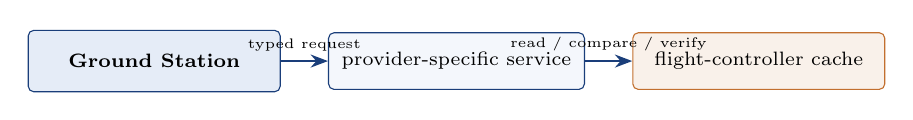
\begin{tikzpicture}[node distance=0.45cm]
  \node[strongbox,minimum width=3.2cm] (gs) {Ground Station};
  \node[box,right=0.6cm of gs,minimum width=3.25cm] (service) {provider-specific service};
  \node[orangebox,right=0.6cm of service,minimum width=3.2cm] (backend) {flight-controller cache};
  \draw[flow] (gs) -- node[above,font=\tiny] {typed request} (service);
  \draw[flow] (service) -- node[above,font=\tiny] {read / compare / verify} (backend);
\end{tikzpicture}
\end{center}
\evidence{VehicleParameterEditRequest/Result; PreflightCheckItem; UavAnalyzeSnapshot}
\end{frame}

\begin{frame}{Live Video: Service Control Opens an Independent Stream}
\footnotesize
\begin{center}
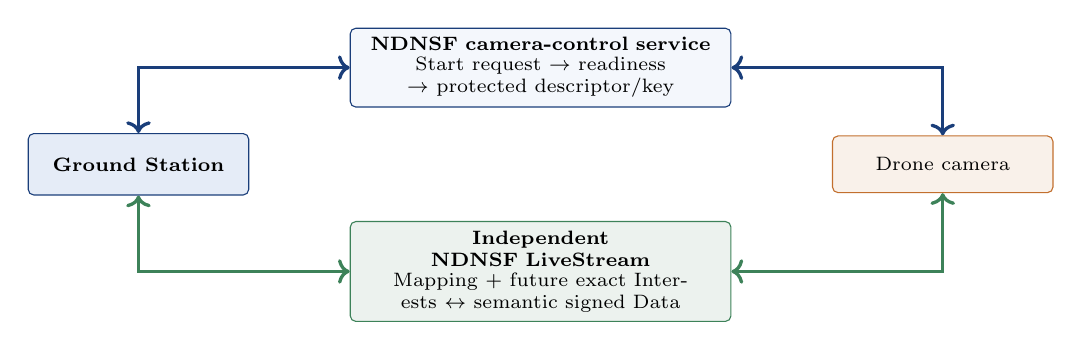
\begin{tikzpicture}[node distance=0.45cm]
  \node[strongbox,minimum width=2.8cm] (gs) {Ground Station};
  \node[orangebox,right=7.4cm of gs,minimum width=2.8cm] (drone) {Drone camera};
  \node[box,above=0.72cm of $(gs)!0.5!(drone)$,text width=4.6cm] (control) {
    \textbf{NDNSF camera-control service}\\[-0.1em]
    \scriptsize Start request $\rightarrow$ readiness $\rightarrow$ protected descriptor/key};
  \node[greenbox,below=0.72cm of $(gs)!0.5!(drone)$,text width=4.6cm] (data) {
    \textbf{Independent NDNSF LiveStream}\\[-0.1em]
    \scriptsize Mapping + future exact Interests $\leftrightarrow$ semantic signed Data};
  \draw[<->,very thick,draw=MemphisBlue] (gs) |- (control);
  \draw[<->,very thick,draw=MemphisBlue] (control) -| (drone);
  \draw[<->,very thick,draw=AccentGreen] (gs) |- (data);
  \draw[<->,very thick,draw=AccentGreen] (data) -| (drone);
\end{tikzpicture}
\end{center}

\vspace{0.55em}
\begin{itemize}
  \item Drone uses \texttt{createLiveStream}; Ground Station uses \texttt{openLiveStream}.
  \item The response authorizes one Stream and returns its descriptor/key; video remains a separate named-data path.
  \item Application lifecycle owns start/stop; Core stop is idempotent and suppresses retired-session callbacks.
\end{itemize}
\evidence{ServiceProvider::createLiveStream; ServiceUser::openLiveStream; Spec 118 camera-start contract}
\end{frame}

\begin{frame}{How Prefetch Preserves Meaningful Data Names}
\scriptsize
\begin{center}
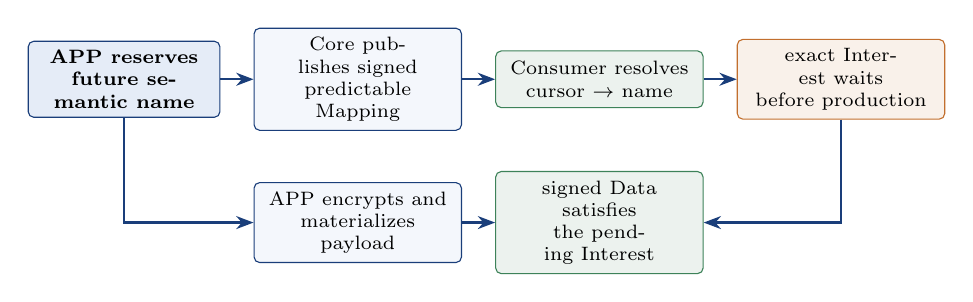
\begin{tikzpicture}[node distance=0.32cm]
  \node[strongbox,text width=2.2cm] (reserve) {APP reserves\\future semantic name};
  \node[box,right=0.42cm of reserve,text width=2.4cm] (map) {Core publishes signed\\predictable Mapping};
  \node[greenbox,right=0.42cm of map,text width=2.4cm] (resolve) {Consumer resolves\\cursor $\rightarrow$ name};
  \node[orangebox,right=0.42cm of resolve,text width=2.4cm] (interest) {exact Interest waits\\before production};
  \draw[flow] (reserve) -- (map);
  \draw[flow] (map) -- (resolve);
  \draw[flow] (resolve) -- (interest);

  \node[box,below=0.65cm of map,text width=2.4cm] (produce) {APP encrypts and\\materializes payload};
  \node[greenbox,right=0.42cm of produce,text width=2.4cm] (return) {signed Data satisfies\\the pending Interest};
  \draw[flow] (reserve) |- (produce);
  \draw[flow] (produce) -- (return);
  \draw[flow] (interest) |- (return);
\end{tikzpicture}
\end{center}

\vspace{0.1em}
\begin{itemize}
  \item Only Mapping names are sequential and constructible; cursor is an internal ordering key.
  \item Payload Data keeps its immutable application name; Mapping carries names, never nested payload Data.
  \item Late Mapping earns no prefetch credit.
\end{itemize}
\bluebox{Predict Mapping, then issue the real semantic-name Interest early: no selector discovery or Data-in-Data encapsulation.}
\evidence{StreamNameMapBlock/Resolver; LiveStreamPublisher::reserveAhead; Spec 119 FR-001/FR-026}
\end{frame}

\begin{frame}{Semantic Name, Encryption, and Session Model}
\footnotesize
\begin{columns}[T]
\begin{column}{0.50\textwidth}
\begin{center}
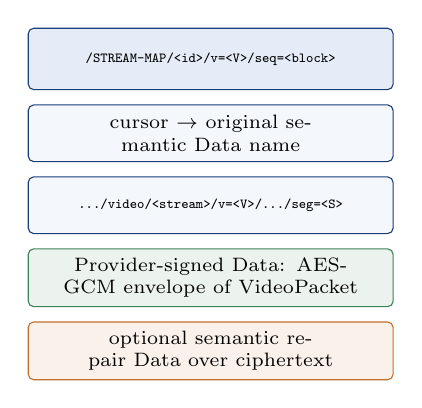
\begin{tikzpicture}[node distance=0.18cm]
  \node[strongbox,text width=4.4cm,font=\tiny] (map) {\texttt{/STREAM-MAP/<id>/v=<V>/seq=<block>}};
  \node[box,below=of map,text width=4.4cm] (binding) {cursor $\rightarrow$ original semantic Data name};
  \node[box,below=of binding,text width=4.4cm,font=\tiny] (name) {\texttt{.../video/<stream>/v=<V>/.../seg=<S>}};
  \node[greenbox,below=of name,text width=4.4cm] (payload) {Provider-signed Data: AES-GCM envelope of VideoPacket};
  \node[orangebox,below=of payload,text width=4.4cm] (fec) {optional semantic repair Data over ciphertext};
\end{tikzpicture}
\end{center}
\end{column}
\begin{column}{0.42\textwidth}
\textbf{Consumer guards}
\begin{itemize}
  \item validate descriptor, Mapping chain, exact name, and expected Provider
  \item authenticate AES-GCM name/session/cursor binding before decode
  \item reject replay, stale session, wrong signer, tag, digest, or nonce
  \item accept recovered opaque bytes only through the same AEAD gate
\end{itemize}

\bluebox{Core never receives the key or plaintext; the cursor never replaces the payload's NDN name.}
\end{column}
\end{columns}
\evidence{UavVideoAad; HybridMessageEnvelope; StreamNameMapBlock; Spec 118}
\end{frame}

\begin{frame}{Paper-Guided Prefetch: Four Receiver Phases}
\scriptsize
\begin{center}
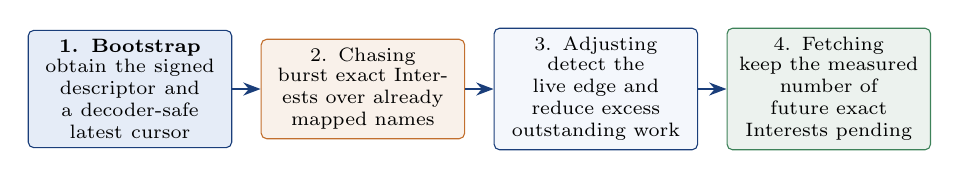
\begin{tikzpicture}[node distance=0.28cm]
  \node[strongbox,text width=2.35cm,minimum height=1.15cm] (boot) {
    1. Bootstrap\\[-0.12em]
    \normalfont obtain the signed descriptor and a decoder-safe latest cursor};
  \node[orangebox,right=0.36cm of boot,text width=2.35cm,minimum height=1.15cm] (chase) {
    2. Chasing\\[-0.12em]
    \normalfont burst exact Interests over already mapped names};
  \node[box,right=0.36cm of chase,text width=2.35cm,minimum height=1.15cm] (adjust) {
    3. Adjusting\\[-0.12em]
    \normalfont detect the live edge and reduce excess outstanding work};
  \node[greenbox,right=0.36cm of adjust,text width=2.35cm,minimum height=1.15cm] (fetch) {
    4. Fetching\\[-0.12em]
    \normalfont keep the measured number of future exact Interests pending};
  \draw[flow] (boot) -- (chase);
  \draw[flow] (chase) -- (adjust);
  \draw[flow] (adjust) -- (fetch);
\end{tikzpicture}
\end{center}

\vspace{0.55em}
\begin{columns}[T]
\begin{column}{0.48\textwidth}
\textbf{Paper's demand estimate}
\[
  D_{sample}=\left\lceil\frac{DRD}{T}\right\rceil
\]
\begin{itemize}
  \item $DRD$: exact Interest expression to matching Data reception
  \item $T$: measured sample production period
\end{itemize}
\end{column}
\begin{column}{0.48\textwidth}
\textbf{NDNSF translation}
\[
  D_{packet}=D_{sample}\!\times\!itemsPerSample+reserve
\]
\begin{itemize}
  \item phase window controls the real cursor horizon
  \item segmented/FEC media keeps one bounded source-group reserve
\end{itemize}
\end{column}
\end{columns}
\evidence{Gusev et al. 2016; LiveStreamPrefetchController; StreamFetchDecision; Spec 123}
\end{frame}

\begin{frame}{The Interest Pipeline Stays Full Before APP Processing}
\scriptsize
\begin{center}
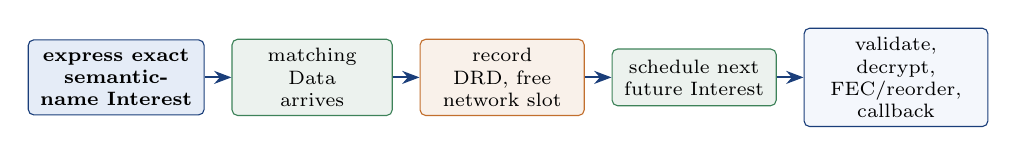
\begin{tikzpicture}[node distance=0.26cm]
  \node[strongbox,text width=2.0cm] (express) {express exact\\semantic-name Interest};
  \node[greenbox,right=0.34cm of express,text width=1.8cm] (receive) {matching Data\\arrives};
  \node[orangebox,right=0.34cm of receive,text width=1.85cm] (refill) {record DRD, free\\network slot};
  \node[greenbox,right=0.34cm of refill,text width=1.85cm] (next) {schedule next\\future Interest};
  \node[box,right=0.34cm of next,text width=2.1cm] (process) {validate, decrypt,\\FEC/reorder, callback};
  \draw[flow] (express) -- (receive);
  \draw[flow] (receive) -- (refill);
  \draw[flow] (refill) -- (next);
  \draw[flow] (next) -- (process);
\end{tikzpicture}
\end{center}

\vspace{0.45em}
\begin{columns}[T]
\begin{column}{0.49\textwidth}
\textbf{Two independent bounded owners}
\begin{itemize}
  \item network in-flight: consumes Interest capacity
  \item payload processing: owns received cursors until APP completion
  \item both sets reject duplicates and drain on stop
\end{itemize}
\end{column}
\begin{column}{0.47\textwidth}
\textbf{Why this matters}
\begin{itemize}
  \item signature validation, decryption, decoding, and GUI work cannot stall Interest refill
  \item a pending exact Interest lets newly produced Data return immediately---approximately one-way network delay, not an extra RTT
\end{itemize}
\end{column}
\end{columns}
\bluebox{Reception refills the network pipeline before APP processing. Prefetch succeeds only when the Provider sees the exact Interest before materializing that Data.}
\evidence{LiveStreamConsumerHandle::schedule; m\_payloadProcessing; payload expression timestamps; Spec 123}
\end{frame}

\begin{frame}{How UAV Video Uses the Generic NDNSF Stream}
\scriptsize
\begin{center}
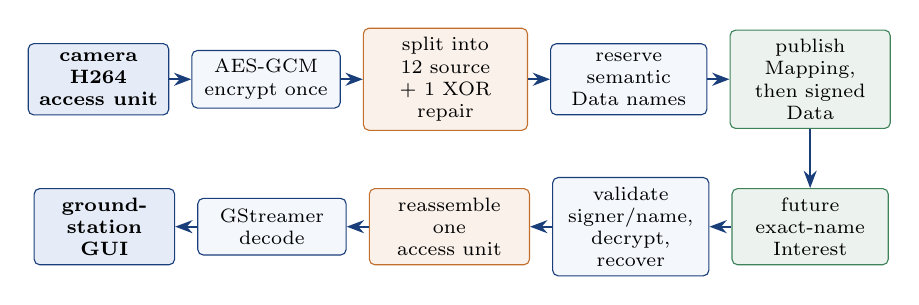
\begin{tikzpicture}[node distance=0.23cm]
  \node[strongbox,text width=1.55cm] (capture) {camera\\H264 access unit};
  \node[box,right=0.28cm of capture,text width=1.65cm] (protect) {AES-GCM\\encrypt once};
  \node[orangebox,right=0.28cm of protect,text width=1.85cm] (split) {split into 12 source\\+ 1 XOR repair};
  \node[box,right=0.28cm of split,text width=1.75cm] (reserve) {reserve semantic\\Data names};
  \node[greenbox,right=0.28cm of reserve,text width=1.8cm] (publish) {publish Mapping,\\then signed Data};
  \draw[flow] (capture) -- (protect);
  \draw[flow] (protect) -- (split);
  \draw[flow] (split) -- (reserve);
  \draw[flow] (reserve) -- (publish);

  \node[greenbox,below=0.75cm of publish,text width=1.75cm] (fetch) {future exact-name\\Interest};
  \node[box,left=0.28cm of fetch,text width=1.75cm] (verify) {validate signer/name,\\decrypt, recover};
  \node[orangebox,left=0.28cm of verify,text width=1.8cm] (assemble) {reassemble one\\access unit};
  \node[box,left=0.28cm of assemble,text width=1.65cm] (decode) {GStreamer\\decode};
  \node[strongbox,left=0.28cm of decode,text width=1.55cm] (display) {ground-station\\GUI};
  \draw[flow] (publish) -- (fetch);
  \draw[flow] (fetch) -- (verify);
  \draw[flow] (verify) -- (assemble);
  \draw[flow] (assemble) -- (decode);
  \draw[flow] (decode) -- (display);
\end{tikzpicture}
\end{center}

\vspace{0.35em}
\begin{itemize}
  \item UAV APP owns H264, 3600-byte packetization, AES-GCM keys/AAD, 12+1 FEC, frame assembly, decoder, and GUI.
  \item NDNSF Core owns signed 32-name Mapping blocks, cursor resolution, exact-name Interests, DRD, phase/window control, bounded retry, ordering, and opaque-byte recovery.
  \item The application Data name remains semantic and Provider-signed; Mapping contains only cursor-to-name bindings, never video payload.
\end{itemize}
\evidence{UavGroundStationApp; UavVideoPipeline; StreamNameMapBlock; LiveStreamPublisher/ConsumerHandle}
\end{frame}

\begin{frame}{What Was Wrong---and What Changed}
\tiny
\renewcommand{\arraystretch}{1.08}
\begin{tabularx}{\textwidth}{p{3.25cm} Y Y}
\toprule
\textbf{Problem} & \textbf{Old behavior} & \textbf{Corrected behavior} \\
\midrule
Delay feedback & capture age treated as network RTT & exact Interest-to-Data DRD only \\
Pipeline refill & waited for validation/decrypt/APP callback & refill immediately on Data reception \\
Phase control & phase/window changed diagnostics only & Chasing/Adjusting window changes actual issued cursors \\
Media demand & one extra packet reserved & one complete 12-packet source group reserved \\
Publisher lifecycle & evicted Data could look ``not produced'' & materialized history distinguishes evicted from future \\
Mapping work & 16 names per signed block & 32 names per block, still about 4.3 KiB \\
Measurement & per-packet DEBUG trace perturbed latency & sampled frame trace retained; packet trace independently disabled \\
\bottomrule
\end{tabularx}

\vspace{0.25em}
\bluebox{This historical Spec 123 failure was prefetch underfill. It is distinct from the later Spec 156 inverse FPS/latency trend, which the next stage-level diagnostic localizes before network fetch/reassembly.}
\evidence{Stream.cpp; TimelineTrace.cpp; Spec 123 evidence sequence}
\end{frame}

\begin{frame}{Corrected 60-Second MiniNDN Result}
\scriptsize
\begin{columns}[T]
\begin{column}{0.52\textwidth}
\renewcommand{\arraystretch}{1.18}
\begin{tabularx}{\linewidth}{Y r}
\toprule
\textbf{Original UAV workload} & \textbf{Measured} \\
\midrule
Video / packetization & 8 Mbps, 3600 B, 12+1 \\
Decoded frames & 1,830 \\
Exact sampled identities & 174/174 (100\%) \\
Decoder startup & 18 ms \\
Capture $\rightarrow$ decode p50 & 142.654 ms \\
Capture $\rightarrow$ decode p95 & 205.946 ms \\
Capture $\rightarrow$ decode p99 & 269.402 ms \\
Decode $\rightarrow$ widget p95 & 4.076 ms \\
\bottomrule
\end{tabularx}
\end{column}
\begin{column}{0.44\textwidth}
\textbf{Network and safety evidence}
\begin{itemize}
  \item Provider future hits: 7,153/7,153
  \item Mapping + payload work: 13.435 Interests/frame
  \item only 3.35\% above the configured 13 stream items/frame
  \item FEC recovered 11 opaque items
  \item rejected correlations: 0
  \item security failures: 0
  \item pending/in-flight at stop: 0/0
\end{itemize}
\end{column}
\end{columns}

\vspace{0.35em}
\bluebox{The original high-packet-rate UAV stream now stays near the live edge; the earlier 1,052 ms result is superseded for this corrected zero-loss configuration.}
\evidence{results/spec123-paper-prefetch-sample-reserve-20260719-060053; Spec 123 completion summary}
\end{frame}

\begin{frame}{Why Higher FPS Shows Lower Latency}
\scriptsize
\begin{columns}[T]
\begin{column}{0.66\textwidth}
  \centering
  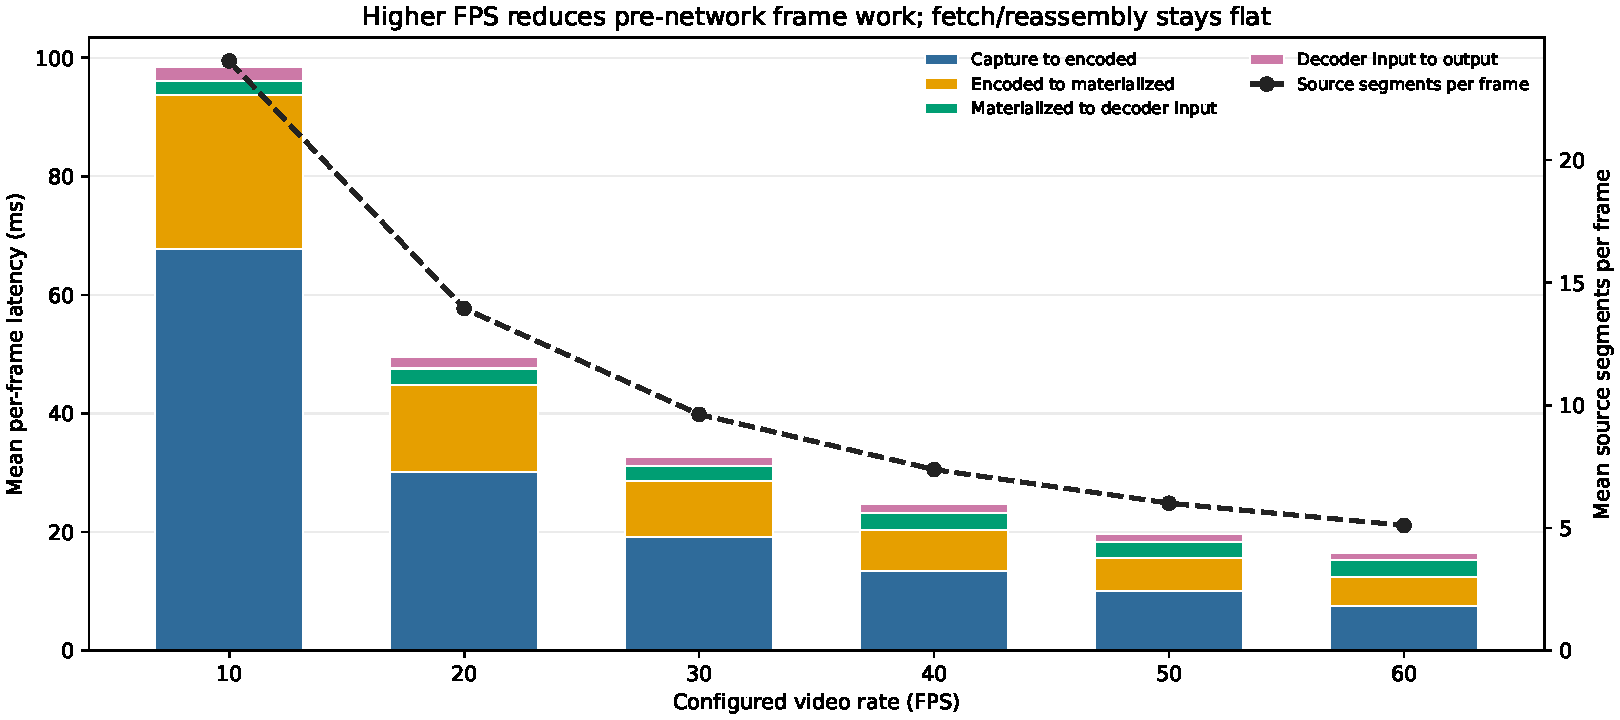
\includegraphics[width=\linewidth]{assets/spec157-stage-latency.pdf}
\end{column}
\begin{column}{0.31\textwidth}
\textbf{Strict per-frame replay}
\begin{itemize}
  \item 15,969/15,969 exact timelines; 100\% coverage
  \item 10$\rightarrow$60 FPS mean end-to-end reduction: 81.923 ms
  \item capture/encode + materialization explain 99.392\% of that reduction
  \item source segments/frame: 24.045$\rightarrow$5.103
  \item materialized$\rightarrow$decoder input: 2.320$\rightarrow$2.884 ms
\end{itemize}
\end{column}
\end{columns}

\vspace{0.25em}
\bluebox{The inverse FPS/latency trend is not evidence of insufficient future Interests: fetch/reassembly does not improve. At fixed bitrate, higher FPS produces smaller frames and less pre-network work per frame.}
\evidence{Spec 157; immutable offline replay of the six Spec 156 cells; no MiniNDN rerun}
\end{frame}

\begin{frame}{Optional XOR Recovery over Opaque Ciphertext}
\footnotesize
\begin{columns}[T]
\begin{column}{0.62\textwidth}
\begin{center}
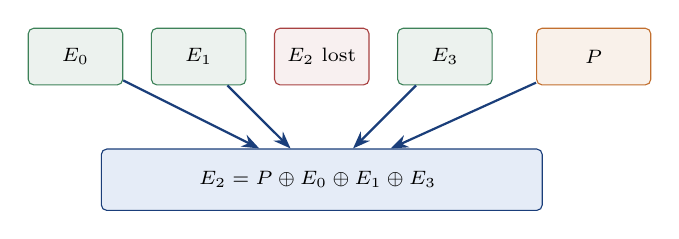
\begin{tikzpicture}[node distance=0.35cm]
  \node[greenbox,minimum width=1.2cm] (d0) {$E_0$};
  \node[greenbox,right=of d0,minimum width=1.2cm] (d1) {$E_1$};
  \node[redbox,right=of d1,minimum width=1.2cm] (d2) {$E_2$ lost};
  \node[greenbox,right=of d2,minimum width=1.2cm] (d3) {$E_3$};
  \node[orangebox,right=0.55cm of d3,minimum width=1.45cm] (p) {$P$};
  \node[strongbox,below=0.8cm of d2,minimum width=5.6cm] (recover) {
    $E_2 = P \oplus E_0 \oplus E_1 \oplus E_3$
  };
  \draw[flow] (d0) -- (recover);
  \draw[flow] (d1) -- (recover);
  \draw[flow] (d3) -- (recover);
  \draw[flow] (p) -- (recover);
\end{tikzpicture}
\end{center}
\end{column}
\begin{column}{0.34\textwidth}
\textbf{Contract v1}
\begin{itemize}
  \item disabled by default; at most one XOR repair item
  \item Core sees encrypted opaque bytes, not H264 plaintext
  \item signed metadata binds Provider, names, lengths, and digests
  \item recovered bytes are AEAD-checked and never cached as original Data
\end{itemize}
\end{column}
\end{columns}

\vspace{0.55em}
\bluebox{One-loss recovery is deterministically correct, but current MiniNDN runs showed no recovery event or performance gain.}
\evidence{LiveStreamFecOptions; publishGroup; FecRecovered provenance; Spec 118/119 evidence}
\end{frame}

\begin{frame}{One Canonical Video Stream, Two Uses}
\footnotesize
\begin{center}
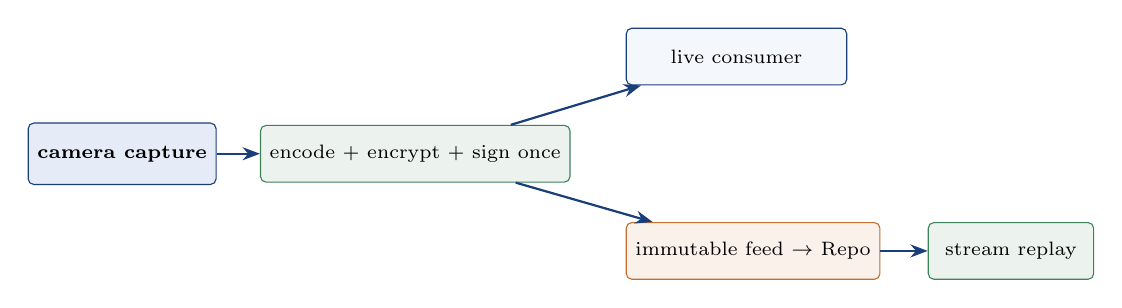
\begin{tikzpicture}[node distance=0.35cm]
  \node[strongbox,minimum width=2.2cm] (camera) {camera capture};
  \node[greenbox,right=0.55cm of camera,minimum width=3.0cm] (publish) {encode + encrypt + sign once};
  \node[box,above right=0.5cm and 0.7cm of publish,minimum width=2.8cm] (viewer) {live consumer};
  \node[orangebox,below right=0.5cm and 0.7cm of publish,minimum width=2.8cm] (repo) {immutable feed $\rightarrow$ Repo};
  \node[greenbox,right=0.6cm of repo,minimum width=2.1cm] (playback) {stream replay};
  \draw[flow] (camera) -- (publish);
  \draw[flow] (publish) -- (viewer);
  \draw[flow] (publish) -- (repo);
  \draw[flow] (repo) -- (playback);
\end{tikzpicture}
\end{center}

\vspace{0.65em}
\begin{itemize}
  \item Viewer and retention lifecycles are independent; the media representation is not.
  \item Repo stores the original semantic name, ciphertext, signature, and wire digest unchanged.
  \item Historical playback reuses normal LiveStream validation, decryption, ordering, and decoding.
\end{itemize}
\evidence{Core PublishedPacketFeed; CanonicalVideoRecordingManifest; Spec 120 acceptance evidence}
\end{frame}

\begin{frame}{Ground-Station Object Detection Callback}
\footnotesize
\begin{center}
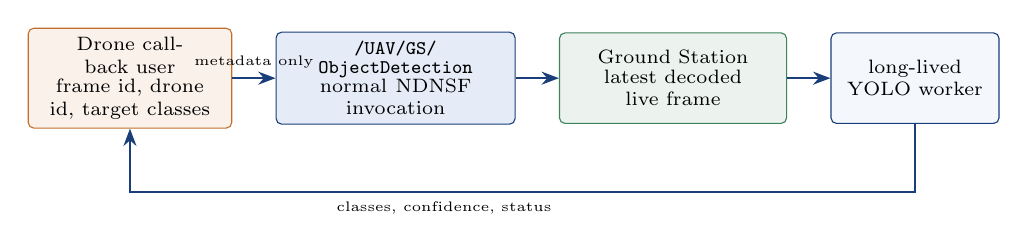
\begin{tikzpicture}[node distance=0.55cm]
  \node[orangebox,text width=2.35cm,minimum height=1.15cm] (drone) {
    Drone callback user\\[-0.1em]
    \normalfont frame id, drone id, target classes
  };
  \node[strongbox,right=0.55cm of drone,text width=2.8cm,minimum height=1.15cm] (service) {
    \texttt{/UAV/GS/}\\[-0.15em]\texttt{ObjectDetection}\\[-0.1em]
    \normalfont normal NDNSF invocation
  };
  \node[greenbox,right=0.55cm of service,text width=2.65cm,minimum height=1.15cm] (frame) {
    Ground Station\\[-0.1em]
    \normalfont latest decoded live frame
  };
  \node[box,right=0.55cm of frame,text width=1.9cm,minimum height=1.15cm] (yolo) {
    long-lived\\YOLO worker
  };
  \draw[flow] (drone) -- node[above,font=\tiny] {metadata only} (service);
  \draw[flow] (service) -- (frame);
  \draw[flow] (frame) -- (yolo);
  \draw[backflow] (drone.south) -- ++(0,-0.8cm) -| node[below,pos=0.2,font=\tiny] {classes, confidence, status} (yolo.south);
\end{tikzpicture}
\end{center}

\vspace{0.7em}
\bluebox{Roles can reverse: a drone is normally a provider, but it can consume a heavier service from the ground station. Image bytes are reused locally and are not inserted into the service request.}
\evidence{installObjectDetectionService; startObjectDetectionLoop; yolo\_detect\_worker.py}
\end{frame}

\begin{frame}{One Runtime, GUI or Headless}
\footnotesize
\begin{columns}[T]
\begin{column}{0.47\textwidth}
\begin{center}
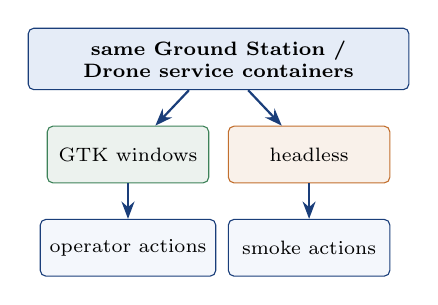
\begin{tikzpicture}[node distance=0.28cm]
  \node[strongbox,text width=4.6cm] (runtime) {same Ground Station / Drone service containers};
  \node[greenbox,below=0.45cm of runtime,xshift=-1.15cm,minimum width=2.05cm] (gui) {GTK windows};
  \node[orangebox,below=0.45cm of runtime,xshift=1.15cm,minimum width=2.05cm] (headless) {headless};
  \node[box,below=0.45cm of gui,minimum width=2.05cm] (human) {operator actions};
  \node[box,below=0.45cm of headless,minimum width=2.05cm] (auto) {smoke actions};
  \draw[flow] (runtime) -- (gui);
  \draw[flow] (runtime) -- (headless);
  \draw[flow] (gui) -- (human);
  \draw[flow] (headless) -- (auto);
\end{tikzpicture}
\end{center}
\end{column}
\begin{column}{0.49\textwidth}
\textbf{Validation layers}
\begin{itemize}
  \item C++ protocol/state unit tests
  \item deployment and config quick smoke
  \item MiniNDN multi-node service tests
  \item PX4 SITL + jMAVSim command/mission tests
  \item GUI smoke under Xvfb
\end{itemize}

\textbf{Default MiniNDN placement}
\begin{itemize}
  \item Controller + GS: Memphis
  \item Drone A: UCLA
  \item Drone B: WUSTL
\end{itemize}
\end{column}
\end{columns}
\evidence{MiniNDN UAV launcher; UAV protocol/state unit tests}
\end{frame}

\begin{frame}{Implemented Foundation and Current Boundary}
\scriptsize
\begin{columns}[T]
\begin{column}{0.49\textwidth}
\textbf{Implemented foundation}
\begin{itemize}
  \item named, permission-controlled UAV services
  \item Targeted command path and typed control state
  \item operator authority and safety gates
  \item multi-drone mission assignment and compensation
  \item semantic-name LiveStream: AES-GCM, signed Mapping, bounded prefetch, optional XOR
  \item encrypted recording discovery and playback
\end{itemize}
\end{column}
\begin{column}{0.47\textwidth}
\textbf{Not yet a production ground station}
\begin{itemize}
  \item complete calibration and firmware setup
  \item full survey/geofence/altitude-profile editing
  \item hardened lost-link and autopilot fail-safe policy
  \item long-duration outdoor and hardware-breadth evidence
  \item certified operator workflow and safety assurance
\end{itemize}
\end{column}
\end{columns}

\vspace{0.25em}
\bluebox{Next: run paired zero-loss and realistic loss/jitter matrices before promoting the corrected future-prefetch profile to the runtime default.}
\evidence{NDNSF-UAV-APP/README.md; Spec 118/119 contracts; Spec 123 completion summary and audit}
\end{frame}

\end{document}
